\subsection{Cálculo de coerência}

Um dos parâmetros mais importantes para o algoritmo LDA é o número de tópicos escondidos que devem ser extraídos do corpus de treinamento.

Sendo o LDA um algoritmo não supervisionado é muito difícil validar se o conjunto de tópicos selecionados para um determinado conjunto de documentos
é útil e faz sentido. Não há uma lista de tópicos corretos previamente selecionados para comparar com os resultados obtidos. Uma forma de medir a 
eficiência do número de tópicos escolhidos é a **coerência**, que é uma avaliação quantitativa da qualidade dos tópicos aprendidos para um determinado 
conjunto de documentos.

Um conjunto de afirmações ou fatos é considerado coerente, se apoiarem um ao outro. Assim, um conjunto de fatos coerente pode ser interpretado 
em um contexto que cobre todos ou a maioria dos fatos. Um exemplo de conjunto de fatos coerentes é “o jogo é um esporte de equipe”, 
“o jogo é jogado com uma bola”, “o jogo exige grandes esforços físicos”.

A coerência de um tópico mede o grau de semelhança semântica entre as palavras que mais contribuem para a definição daquele tópico.
Esta medida ajuda a distinguir entre os tópicos que são \textbf{semanticamente interpretáveis} e os tópicos que são 
\textbf{artefatos de inferência estatística}.

Há várias medidas de coerência e a que escolhi foi a \textbf{c\_v}. Na lista de referências há artigos que explicam esta e outras 
medidas de coerência. O que importa é que um maior valor indica maior coerência.

\subsubsection{Análise de coerências}

Conforme podemos ver código fonte na seção seguinte, há alguns parâmetros importantes para o cálculo da coerência:

\begin{itemize}
    \item \textbf{documents}: lista de documentos que compôem nosso corpus
    \item \textbf{num\_topics}: número de tópicos para os quais queremos calcular a coerência
\end{itemize}

Apesar de não ser explicitamente utilizados no código, os parâmetros \textbf{alpha} e \textbf{eta} mencionados anteriormente são também importantes mas neste cálculo inicial
optei por mantê-los em seu valor padrão, que é 1/número de tópicos. 

A lista de documentos contempla o conjunto completo de textos de nossa fonte de dados de origem. O número de tópicos eu variei entre 5 e 120, de um 
a um. O resultado gerado foi um arquivo csv contendo os seguintes campos:

\begin{itemize}
    \item num\_topics: número de tópicos no Treinamento
    \item coherence: coerência para aquele número de tópicos
    \item tempo\_gasto: tempo total gasto no cálculo de coerência para o número de tópicos
\end{itemize}

Com base no resultado dos cálculos das coerências para o número de tópicos foi gerado o gráfico a seguir, onde já podemos ver que a coerência para 
de crescer e de certa forma e começa a oscilar para cima e para baixo sem grandes variações a partir de um determinado número de tópicos.

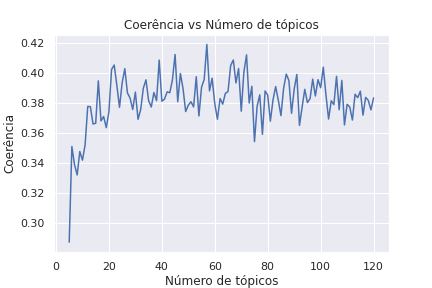
\includegraphics{treinamento/resources/coerencia_vs_topicos.png}

Ordenando os valores das coerências nós obtemos as dez maiores e seus respectivos tópicos, conforme vemos abaixo ordenando começando pela maior.

\begin{center}
\begin{tabular}{ |c|c| }
 \hline
 Número de tópicos & Coerência \\ [0.5ex]
 \hline\hline
 57 & 0.4187279439804192 \\
 45 & 0.4120513470103957 \\
 72 & 0.4118140382511174 \\
 67 & 0.4084148429857527 \\
 39 & 0.4083294457749056 \\
 22 & 0.4050952035903351 \\
 66 & 0.4047401968259075 \\
 101 & 0.4036451569534363 \\
 69 & 0.4027847252786048 \\
 26 & 0.4026587678111619 \\
 \hline
\end{tabular}
\end{center}

Abaixo segue uma listagem com o código fonte usado para o cálculo das coerências para um conjunto de documentos e intervalo de números de tópicos.

\subsubsection{Código fonte}

\lstinputlisting[language=Python, style=mystyle, frame=lines, caption=Código fonte: Cálculo de coerência de tópicos]{resources/coerencia.py}